\chapter{Implementaci�n}
\label{cap:implementacionDelTFG}

\section{Herramientas utilizadas}
La implementaci�n de esta aplicaci�n se ha llevado a cabo con la siguientes herramientas:
\begin{itemize}
	\item Para el front-end de la aplicaci�n hemos utilizado HTML y CSS por la facilidad de uso y generaci�n de c�digo. Tambi�n, hemos incorporado Bootstrap para los estilos de la aplicaci�n ya que simplifica la generaci�n de formulario. Adem�s, Bootstrap genera c�digo Responsive que es uno de los requisitos para poder utilizar la aplicaci�n en tablets. Para la conexi�n con el Back hemos utilizado JavaScript por sencillez y porque es un lenguaje que conocemos todos los integrantes del grupo.
	\item Para el back-end hemos utilizado PHP porque lo hemos utilizado en otras asignaturas y nos resulta muy familiar.
	\item Para almacenar los datos hemos utilizado el motor de base de datos MySQL porque es de c�digo abierto.
	\item Como servidor local hemos utilizado Xampp porque es un servidor de plataforma libre y nos da muchas facilidades porque integra varias aplicaciones (MySQL, PHP). Adem�s, se puede ejecutar en diversos sistemas operativos que nos ha facilitado colaborar en equipo.
	\item Como herramienta de control de versiones hemos utilizao GitHub ya que es donde alojamos todo el material del TFG.
	\item Para desarrollar la aplicaci�n utilizamos  Visual Studio Code como editor de c�digo puesto que consideramos que es el m�s completo y con el que m�s familiarizados estamos.
\end{itemize}

\section{Estructura de la Base de datos}
Hemos dise�ado un modelo de base de datos relacional (ver Figura \ref{fig:estructura-bd}).
\begin{figure}[!ht]
  	\centering
  	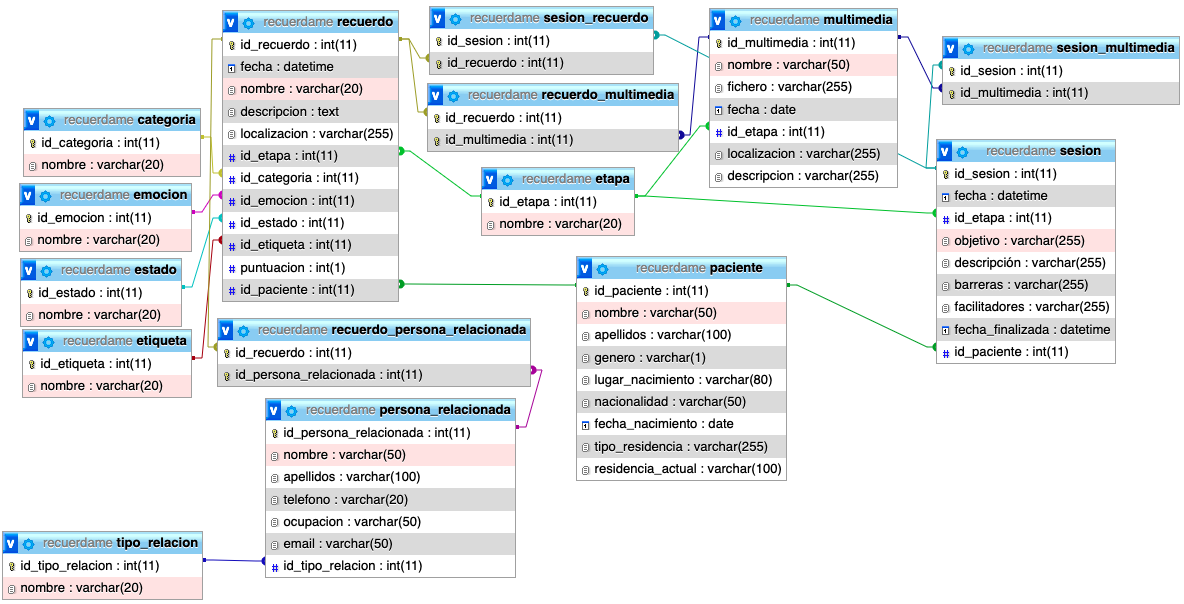
\includegraphics[width=16cm]{./Imagenes/Figuras/estructura-bd}
  	\caption{Estructura de la base de datos.}
	\label{fig:estructura-bd}
\end{figure}